\documentclass[11pt,a4paper]{article}
\usepackage[utf8]{inputenc}
\usepackage{amsmath,amssymb,amsfonts}
\usepackage{graphicx}
\usepackage{booktabs}
\usepackage{tabularx}
\usepackage{geometry}
\geometry{margin=1in}
\usepackage{hyperref}
\hypersetup{
    colorlinks=true,
    linkcolor=blue,
    citecolor=blue,
    urlcolor=blue
}

\title{\textbf{Supplementary Material:\\A Controlled Empirical Comparison of Classical and Quantum Kernel SVMs for Breast Cancer Classification}}
\author{\textbf{Sina Qasempour}\\[1ex]\textit{Independent Researcher, Iran}\\\textit{Corresponding author: qasempoursina@gmail.com}\\\textit{ORCID: \url{https://orcid.org/0009-0006-8853-6740}}}
\date{September 2026}

\begin{document}

\renewcommand{\thetable}{S\arabic{table}}
\renewcommand{\thefigure}{S\arabic{figure}}

\maketitle

\noindent\textbf{Provenance:} historical release \texttt{v1.0.0}; corrected checkpoint \texttt{f4c8418}\\
\noindent\textbf{Repository:} \url{https://github.com/SinaQP/SVM-Vs-QSVM}\\
\noindent\textbf{Primary Endpoint:} Malignant Class F1 Score (\texttt{pos\_label=0})

\bigskip
\hrule
\bigskip

\section*{Supplementary Section S0: Corrected Nested QSVC Selection}

For each predefined outer seed, the authoritative QSVC procedure used five-fold stratified inner cross-validation confined to the 455-sample outer-training set. \texttt{StandardScaler}, PCA, \texttt{MinMaxScaler([0,$\pi$])}, statevectors, and training/validation Gram matrices were recomputed within every inner fold. The joint grid was $\text{reps}\in\{1,2,3\}$ and $C\in\{0.01,0.1,1,10,100\}$; 4Q additionally searched linear and full entanglement. For 2Q, the topology labels are algebraically equivalent because there is only one qubit pair, so linear is the single canonical representative. Selection maximized mean inner-fold malignant-class F1; ties favored lower repetitions, then linear, then smaller $C$. The chosen configuration was frozen before full outer-train refitting and one outer-test evaluation.

\begin{table}[htbp]
\centering
\caption{Per-seed corrected nested QSVC selections.}
\begin{tabular}{ccccc}
\toprule
Outer seed & Representation & Reps & Topology & $C$ \\
\midrule
42 & PCA 2 / 2Q & 1 & linear & 100 \\
123 & PCA 2 / 2Q & 1 & linear & 100 \\
456 & PCA 2 / 2Q & 1 & linear & 1 \\
789 & PCA 2 / 2Q & 1 & linear & 10 \\
2026 & PCA 2 / 2Q & 1 & linear & 10 \\
42, 123, 456, 789, 2026 & PCA 4 / 4Q & 1 & full & 1 \\
\bottomrule
\end{tabular}
\end{table}

Across the ten representation/seed selections, one repetition was selected 10/10 times; two and three repetitions were each selected 0/10 times. In 4Q, full was selected 5/5 times and linear 0/5 times. This nested search is the source of the final QSVC models. The separate outer-test ablation remains an exploratory sensitivity analysis and did not choose these configurations.

\section*{Supplementary Section S1: Extended Sample-Size Scaling Evaluation}

Models were trained on nested subsets $N_{\text{train}} \in \{50, 100, 200, 300, 455\}$ with preprocessing pipelines (\texttt{StandardScaler}, \texttt{PCA}, \texttt{MinMaxScaler}) independently refit on each subset and evaluated on fixed outer test partitions ($N_{\text{test}}=114$). All learning curves use fixed classifier settings: $C=1$ for every SVC, \texttt{gamma='scale'} for RBF, and \texttt{reps}=1 with full entanglement for QSVC. They are separate from the authoritative nested-selected comparison.

\begin{table}[htbp]
\centering
\caption{Complete Sample-Size Scaling Results across 5 Outer Splits (Mean $\pm$ SD).}
\label{tab:supp_scaling}
\vspace{2mm}
\resizebox{\textwidth}{!}{%
\begin{tabular}{lllccccccc}
\toprule
$N_{\text{train}}$ & Model Architecture & Family & Repr. & Qubits & Test Accuracy & Precision & Recall & Malignant F1 & ROC-AUC \\
\midrule
\textbf{50} & Linear SVM & Classical & PCA 2 & 0 & $0.9333 \pm 0.0354$ & $0.8726 \pm 0.0699$ & $0.9667 \pm 0.0271$ & $\mathbf{0.9157 \pm 0.0402}$ & $0.9874 \pm 0.0087$ \\
50 & RBF SVM & Classical & PCA 2 & 0 & $0.9263 \pm 0.0282$ & $0.9006 \pm 0.0603$ & $0.9048 \pm 0.0532$ & $0.9008 \pm 0.0353$ & $0.9839 \pm 0.0072$ \\
50 & QSVC (reps=1, full) & Quantum & PCA 2 & 2 & $0.8246 \pm 0.0387$ & $0.8242 \pm 0.0957$ & $0.6762 \pm 0.0643$ & $\mathbf{0.7398 \pm 0.0531}$ & $0.8850 \pm 0.0484$ \\
\addlinespace
50 & Linear SVM & Classical & PCA 4 & 0 & $0.9316 \pm 0.0353$ & $0.8857 \pm 0.0893$ & $0.9476 \pm 0.0261$ & $\mathbf{0.9128 \pm 0.0395}$ & $0.9894 \pm 0.0090$ \\
50 & RBF SVM & Classical & PCA 4 & 0 & $0.9421 \pm 0.0295$ & $0.9197 \pm 0.0607$ & $0.9286 \pm 0.0558$ & $0.9222 \pm 0.0385$ & $0.9864 \pm 0.0060$ \\
50 & QSVC (reps=1, full) & Quantum & PCA 4 & 4 & $0.7263 \pm 0.0716$ & $0.6931 \pm 0.1444$ & $0.4095 \pm 0.2146$ & $\mathbf{0.4994 \pm 0.2110}$ & $0.7636 \pm 0.1082$ \\
\midrule
\textbf{100} & Linear SVM & Classical & PCA 2 & 0 & $0.9474 \pm 0.0175$ & $0.9311 \pm 0.0454$ & $0.9286 \pm 0.0412$ & $\mathbf{0.9287 \pm 0.0227}$ & $0.9884 \pm 0.0067$ \\
100 & RBF SVM & Classical & PCA 2 & 0 & $0.9246 \pm 0.0237$ & $0.9086 \pm 0.0585$ & $0.8905 \pm 0.0686$ & $0.8966 \pm 0.0317$ & $0.9849 \pm 0.0092$ \\
100 & QSVC (reps=1, full) & Quantum & PCA 2 & 2 & $0.8614 \pm 0.0190$ & $0.8679 \pm 0.0647$ & $0.7429 \pm 0.0391$ & $\mathbf{0.7983 \pm 0.0207}$ & $0.9214 \pm 0.0101$ \\
\addlinespace
100 & Linear SVM & Classical & PCA 4 & 0 & $0.9421 \pm 0.0288$ & $0.9246 \pm 0.0675$ & $0.9238 \pm 0.0488$ & $\mathbf{0.9222 \pm 0.0355}$ & $0.9890 \pm 0.0074$ \\
100 & RBF SVM & Classical & PCA 4 & 0 & $0.9386 \pm 0.0139$ & $0.9256 \pm 0.0380$ & $0.9095 \pm 0.0639$ & $0.9155 \pm 0.0217$ & $0.9884 \pm 0.0044$ \\
100 & QSVC (reps=1, full) & Quantum & PCA 4 & 4 & $0.7947 \pm 0.0332$ & $0.8059 \pm 0.0713$ & $0.6048 \pm 0.1722$ & $\mathbf{0.6733 \pm 0.0978}$ & $0.8628 \pm 0.0326$ \\
\midrule
\textbf{200} & Linear SVM & Classical & PCA 2 & 0 & $0.9421 \pm 0.0159$ & $0.9008 \pm 0.0237$ & $0.9476 \pm 0.0310$ & $\mathbf{0.9234 \pm 0.0213}$ & $0.9867 \pm 0.0079$ \\
200 & RBF SVM & Classical & PCA 2 & 0 & $0.9316 \pm 0.0157$ & $0.9157 \pm 0.0451$ & $0.9000 \pm 0.0391$ & $0.9066 \pm 0.0202$ & $0.9864 \pm 0.0045$ \\
200 & QSVC (reps=1, full) & Quantum & PCA 2 & 2 & $0.8877 \pm 0.0144$ & $0.8821 \pm 0.0521$ & $0.8095 \pm 0.0753$ & $\mathbf{0.8406 \pm 0.0259}$ & $0.9453 \pm 0.0115$ \\
\addlinespace
200 & Linear SVM & Classical & PCA 4 & 0 & $0.9579 \pm 0.0157$ & $0.9432 \pm 0.0262$ & $0.9429 \pm 0.0213$ & $\mathbf{0.9429 \pm 0.0210}$ & $0.9910 \pm 0.0029$ \\
200 & RBF SVM & Classical & PCA 4 & 0 & $0.9509 \pm 0.0159$ & $0.9311 \pm 0.0382$ & $0.9381 \pm 0.0398$ & $0.9337 \pm 0.0216$ & $0.9907 \pm 0.0047$ \\
200 & QSVC (reps=1, full) & Quantum & PCA 4 & 4 & $0.8579 \pm 0.0287$ & $0.8532 \pm 0.0598$ & $0.7476 \pm 0.0686$ & $\mathbf{0.7943 \pm 0.0440}$ & $0.9298 \pm 0.0148$ \\
\midrule
\textbf{300} & Linear SVM & Classical & PCA 2 & 0 & $0.9439 \pm 0.0268$ & $0.9118 \pm 0.0589$ & $0.9429 \pm 0.0361$ & $\mathbf{0.9258 \pm 0.0328}$ & $0.9892 \pm 0.0038$ \\
300 & RBF SVM & Classical & PCA 2 & 0 & $0.9333 \pm 0.0133$ & $0.9242 \pm 0.0403$ & $0.8952 \pm 0.0494$ & $0.9080 \pm 0.0191$ & $0.9864 \pm 0.0047$ \\
300 & QSVC (reps=1, full) & Quantum & PCA 2 & 2 & $0.9158 \pm 0.0260$ & $0.9193 \pm 0.0448$ & $0.8476 \pm 0.0598$ & $\mathbf{0.8807 \pm 0.0388}$ & $0.9651 \pm 0.0130$ \\
\addlinespace
300 & Linear SVM & Classical & PCA 4 & 0 & $0.9596 \pm 0.0078$ & $0.9441 \pm 0.0240$ & $0.9476 \pm 0.0310$ & $\mathbf{0.9453 \pm 0.0112}$ & $0.9943 \pm 0.0019$ \\
300 & RBF SVM & Classical & PCA 4 & 0 & $0.9544 \pm 0.0144$ & $0.9493 \pm 0.0444$ & $0.9286 \pm 0.0376$ & $0.9377 \pm 0.0188$ & $0.9936 \pm 0.0037$ \\
300 & QSVC (reps=1, full) & Quantum & PCA 4 & 4 & $0.8877 \pm 0.0259$ & $0.8725 \pm 0.0539$ & $0.8190 \pm 0.0598$ & $\mathbf{0.8429 \pm 0.0351}$ & $0.9489 \pm 0.0156$ \\
\midrule
\textbf{455} & Linear SVM & Classical & PCA 2 & 0 & $0.9474 \pm 0.0152$ & $0.9152 \pm 0.0444$ & $0.9476 \pm 0.0261$ & $\mathbf{0.9302 \pm 0.0182}$ & $0.9897 \pm 0.0026$ \\
455 & RBF SVM & Classical & PCA 2 & 0 & $0.9439 \pm 0.0159$ & $0.9339 \pm 0.0411$ & $0.9143 \pm 0.0271$ & $0.9233 \pm 0.0202$ & $0.9864 \pm 0.0040$ \\
455 & QSVC (reps=1, full) & Quantum & PCA 2 & 2 & $0.9123 \pm 0.0224$ & $0.9313 \pm 0.0269$ & $0.8238 \pm 0.0706$ & $\mathbf{0.8726 \pm 0.0376}$ & $0.9697 \pm 0.0141$ \\
\addlinespace
455 & Linear SVM & Classical & PCA 4 & 0 & $0.9632 \pm 0.0157$ & $0.9493 \pm 0.0344$ & $0.9524 \pm 0.0376$ & $\mathbf{0.9501 \pm 0.0211}$ & $0.9952 \pm 0.0030$ \\
455 & RBF SVM & Classical & PCA 4 & 0 & $0.9579 \pm 0.0200$ & $0.9448 \pm 0.0436$ & $0.9429 \pm 0.0361$ & $0.9430 \pm 0.0259$ & $0.9944 \pm 0.0035$ \\
455 & QSVC (reps=1, full) & Quantum & PCA 4 & 4 & $0.9053 \pm 0.0423$ & $0.8748 \pm 0.0767$ & $0.8762 \pm 0.0832$ & $\mathbf{0.8721 \pm 0.0556}$ & $0.9581 \pm 0.0227$ \\
\bottomrule
\end{tabular}%
}
\end{table}

\newpage
\section*{Supplementary Section S2: Computational Complexity and Execution Profiling}

The reported \texttt{total\_runtime} includes preprocessing, classifier fitting, and prediction; QSVC additionally includes exact statevector generation and both training and test Gram products. Inner-search and kernel-diagnostic time are excluded.

\begin{table}[htbp]
\centering
\caption{Execution Time, Computational Complexity, and Storage Footprint.}
\label{tab:supp_runtime}
\vspace{2mm}
\resizebox{\textwidth}{!}{%
\begin{tabular}{llccccc}
\toprule
Pipeline Stage / Architecture & Platform & Qubits & Mean Runtime (s) & Rel. Cost & Time Complexity & Memory Complexity \\
\midrule
Linear SVM (PCA 2) & CPU LibSVM & 0 & $0.0048 \pm 0.0007$ & $1.0\times$ (Ref) & $\mathcal{O}(dN_{tr}^2)$--$\mathcal{O}(dN_{tr}^3)$, data dependent & Data/cache dependent \\
RBF SVM (PCA 2) & CPU LibSVM & 0 & $0.0072 \pm 0.0024$ & $1.5\times$ & Same SVC bounds; pairwise RBF work & Data/cache dependent \\
Linear SVM (PCA 4) & CPU LibSVM & 0 & $0.0083 \pm 0.0061$ & $1.7\times$ & $\mathcal{O}(dN_{tr}^2)$--$\mathcal{O}(dN_{tr}^3)$, data dependent & Data/cache dependent \\
RBF SVM (PCA 4) & CPU LibSVM & 0 & $0.0071 \pm 0.0019$ & $1.5\times$ & Same SVC bounds; pairwise RBF work & Data/cache dependent \\
QSVC (2Q Statevector) & Vectorized CPU & 2 & $0.2181 \pm 0.0096$ & $\sim 45\times$ & $\mathcal{O}((N_{tr}^2+N_{te}N_{tr})2^q)$ plus SVC & Train+test kernels: 2,071,160 B \\
QSVC (4Q Statevector) & Vectorized CPU & 4 & $0.5846 \pm 0.0257$ & $\sim 71\times$ & Same form with larger $q$ plus SVC & Train+test kernels: 2,071,160 B \\
\midrule
\textit{Historical 2Q ComputeUncompute} & Local circuit-pair sampler & 2 & $120.5 \pm 15.2$ & $\sim 25,000\times$ & $\mathcal{O}(N_{tr}^2+N_{te}N_{tr})$ pairs & Train+test Gram arrays \\
\textit{Historical 4Q ComputeUncompute} & Local circuit-pair sampler & 4 & $455.0 \pm 40.0$ & $\sim 55,000\times$ & $\mathcal{O}(N_{tr}^2+N_{te}N_{tr})$ pairs & Train+test Gram arrays \\
\bottomrule
\end{tabular}%
}
\end{table}

The exact statevector and historical \texttt{ComputeUncompute} measurements are separate CPU-simulation regimes. Neither is a physical-QPU timing, and no fixed hardware shot budget is inferred.

\bigskip

\section*{Supplementary Section S3: Supplementary Diagnostic Figures}

\begin{figure}[htbp]
\centering
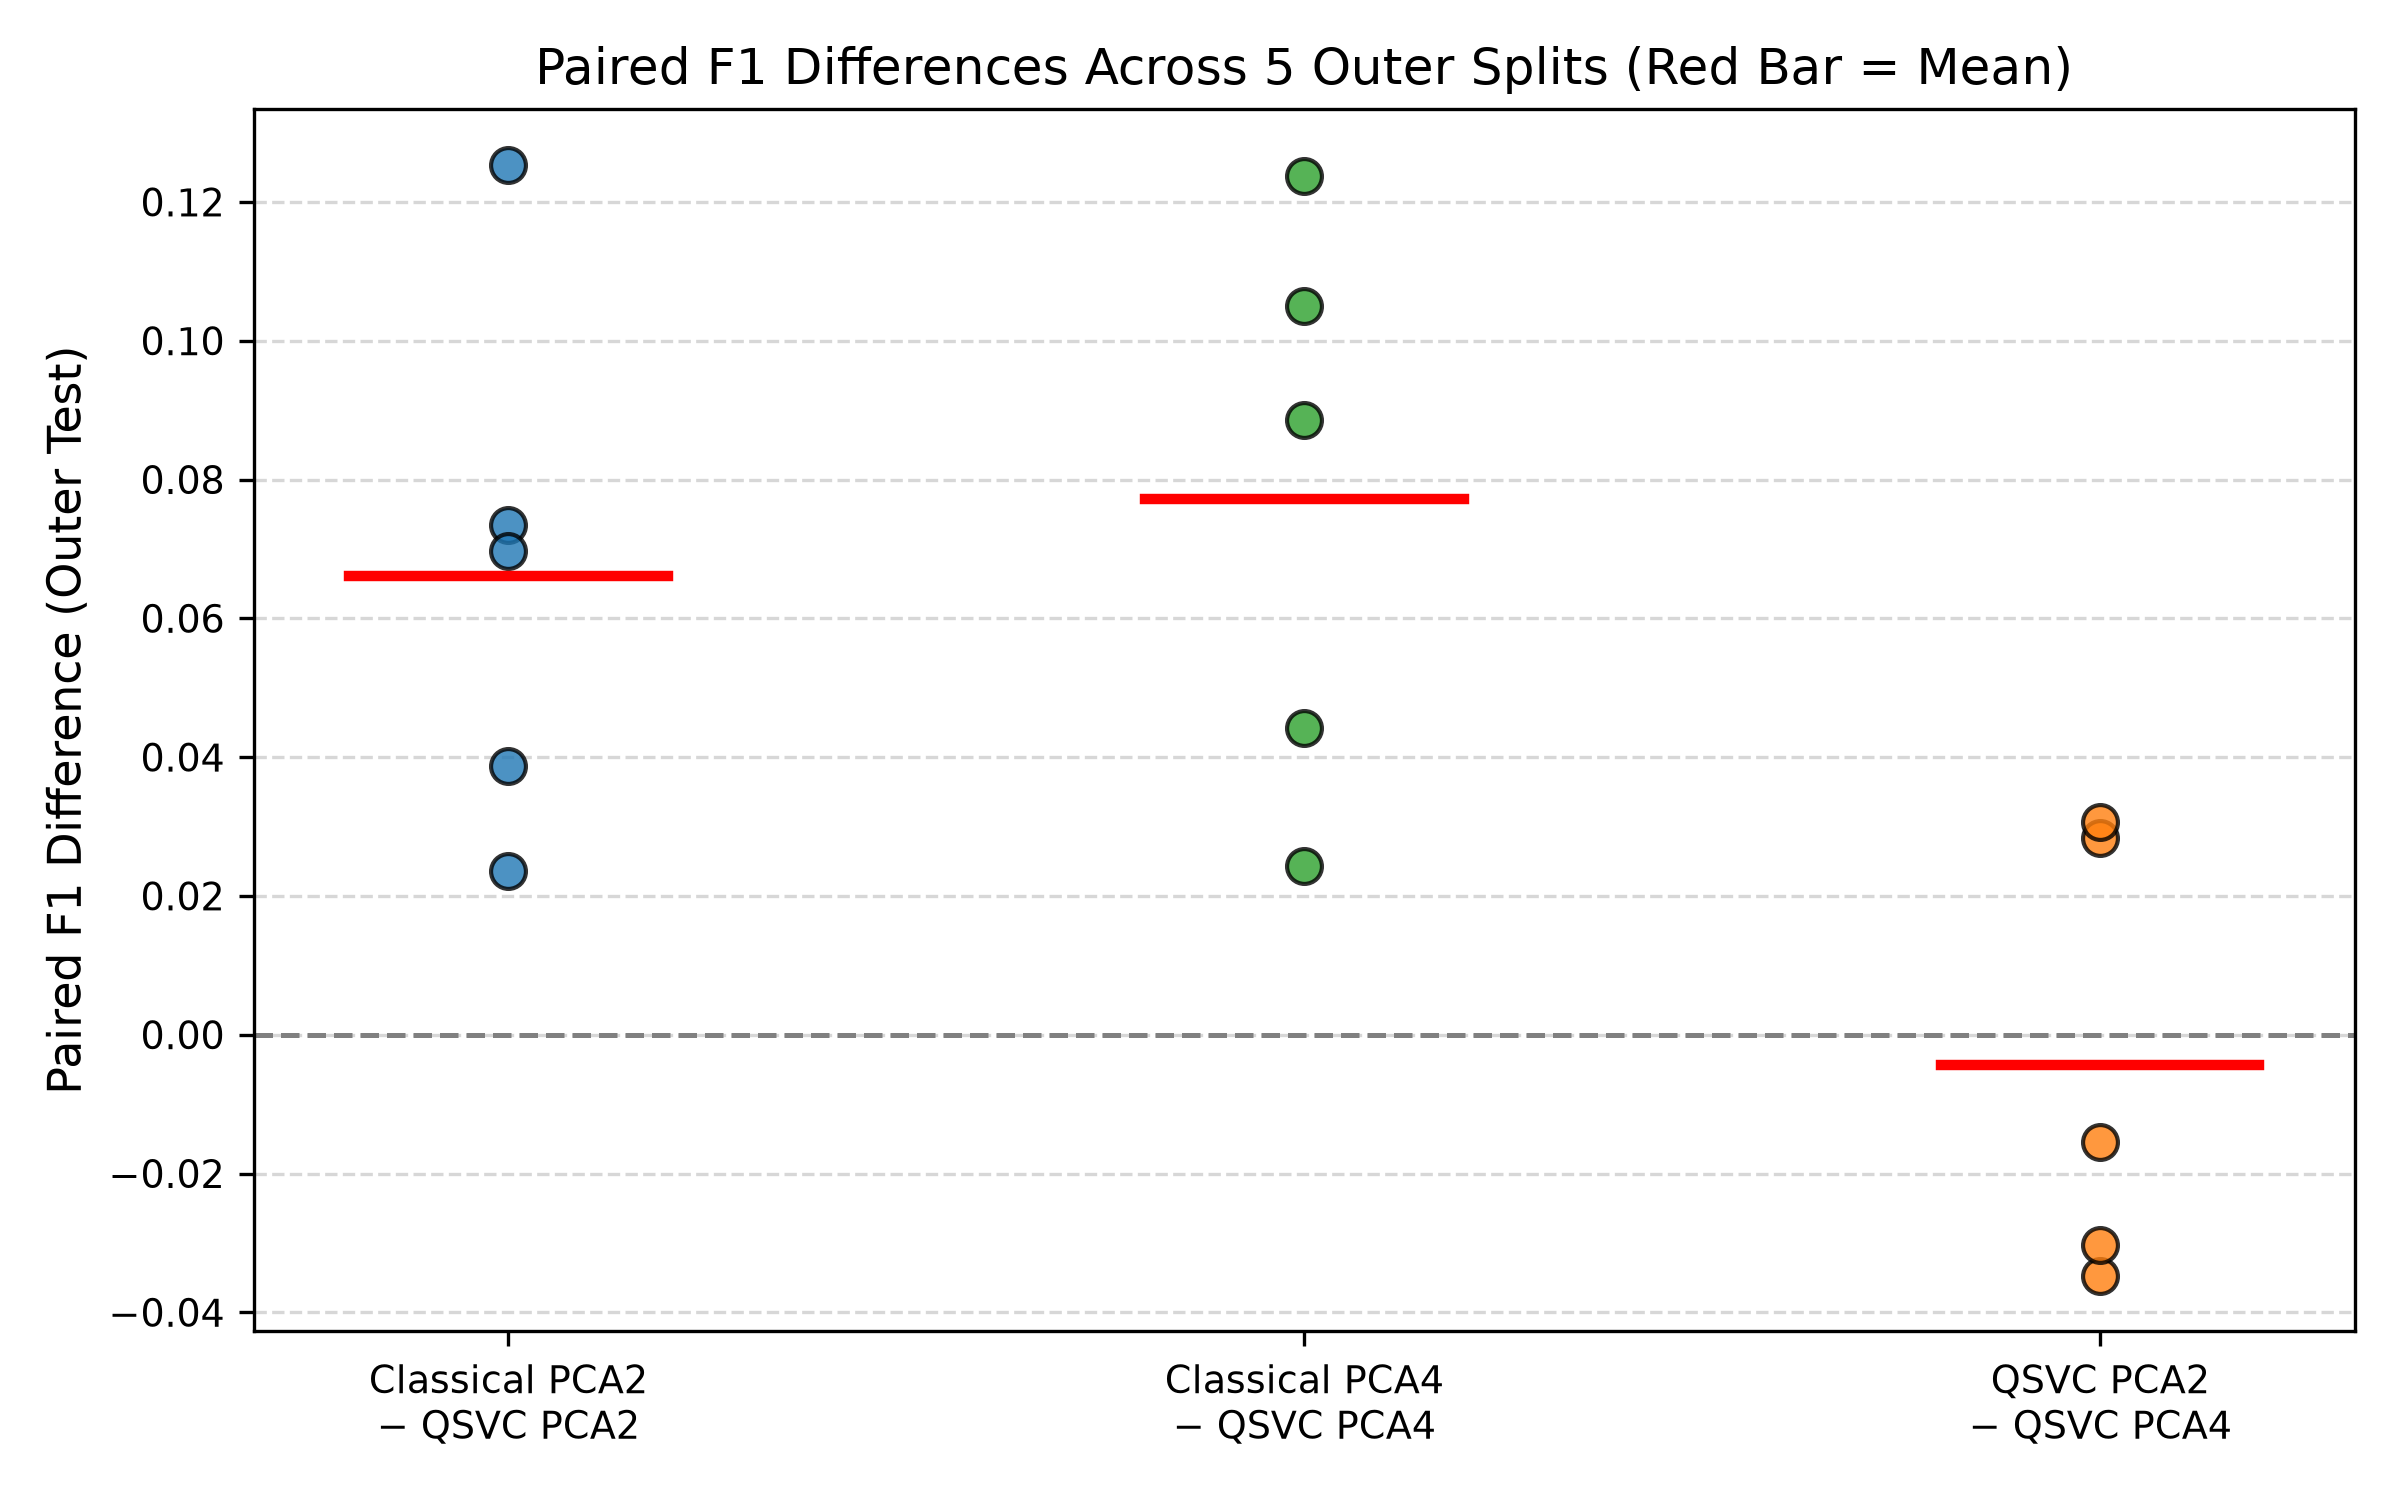
\includegraphics[width=0.85\textwidth]{final_paired_f1_differences.png}
\caption{\textbf{Paired Split-Level F1 Differences.} Distribution of paired differences $\Delta = \text{F1}_{\text{Classical}} - \text{F1}_{\text{QSVC}}$ across five outer test splits. Classical models achieve higher malignant F1 scores on 5/5 splits in both PCA 2 and PCA 4 representations.}
\label{fig:supp_paired}
\end{figure}

\begin{figure}[htbp]
\centering
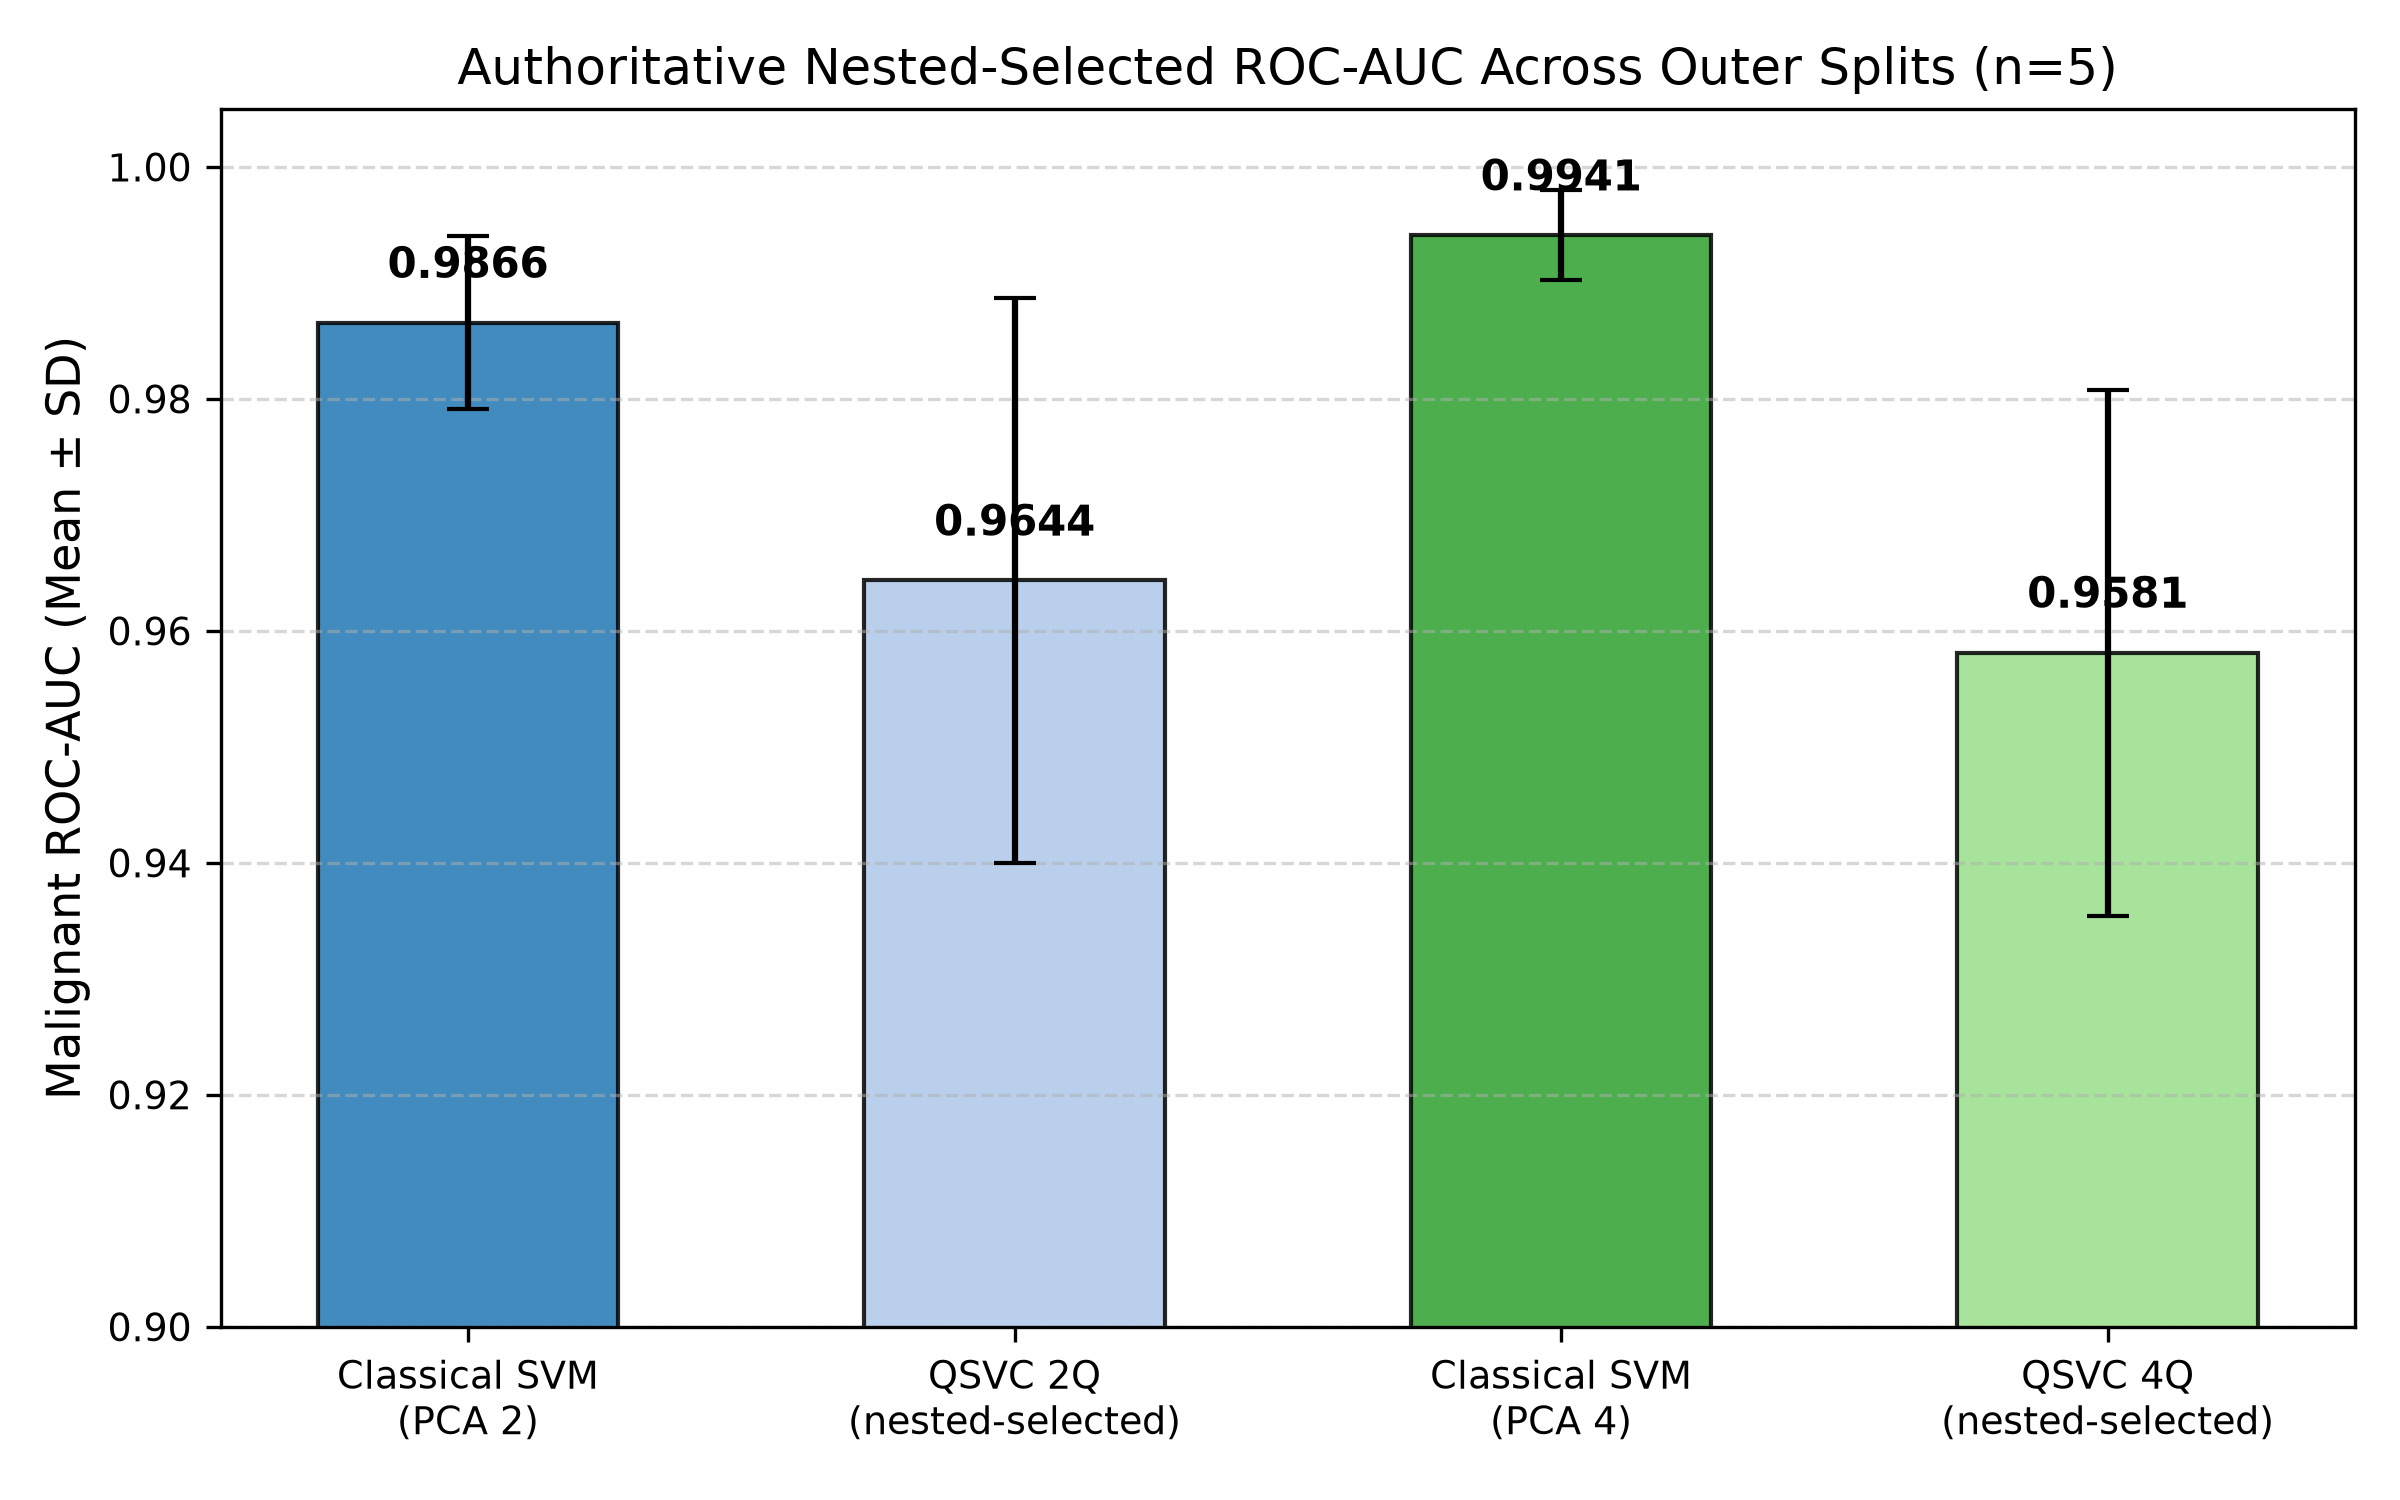
\includegraphics[width=0.85\textwidth]{final_roc_auc_comparison.png}
\caption{\textbf{Outer-Test ROC-AUC Comparison.} Mean receiver operating characteristic area under curve across five outer splits comparing classical and quantum models.}
\label{fig:supp_roc}
\end{figure}

\end{document}
